%%\section{Formal verification according to ISO~26262}
%% TODO: write what formal/semi-formal verification means according to ISO.

\section{Achieving good test cases}
To find good test cases is not trivial. It may not be enough to
generate test cases which follows a correct behavior. Negative testing
also needs to be taken into consideration.

\subsection{Negative Testing}
The problem with negative testing is that the watchdog manager quickly
will be put in an absorbing state when an invalid API-call is
executed. After such an invalid execution, all following API-calls
will not test anything new since the absorbing state is reached. As a
consequence it is not possible to test multiple invalid executions
with one test. A problem using QuickCheck is that the test cases are
generated before the actual execution of the program; it is likely
that a lot of API-calls will be executed after an invalid execution of
the program. This results in that negative testing may be time
consuming using QuickCheck.

\subsection{Positive Testing}
There are a lot of things that can cause an invalid behavior of the
watchdog manager. Because of this, there may be a lot of calculations
needed to find test cases that are valid, so that the absorbing state
is not reached. The complexity of finding such cases grows with the
complexity of the configuration. However, properties are continuously
tested as long the absorbing state is not reached. Eventually, even
when trying to make use of positive testing, the absorbing state will
be reached if the configuration is not to simple. This is because the
order of commands will influence if the behavior is correct or
not. Even if it is possible to prioritize certain commands the random
factor of QuickCheck will eventually cause an invalid behavior. See
figure \ref{FIG:STATUSES_BSI}, \ref{FIG:STATUSES_FREESCALE}, and
\ref{FIG:STATUSES_EXAMPLE} for how many commands that are executed
before the absorbing state \lstinline!'WDGM_GLOBAL_STATUS_EXPIRED'! is
reached.

\subsection{Prioritized Testing}
The supervision algorithms are important parts of the watchdog manager
since they specify transitions, liveness and timing properties of the
program. It was therefore chosen to prioritize different algorithms
when running some of the tests on the module. When doing so, more bugs
were found. This emphasizes the importance of finding tests that are
critical for the system and not lean the results only on line
coverage.

Since there are different supervisions of checkpoints that can be
configured at the same time, the supervision functions must be
prioritized when generating command sequences and arguments. A
checkpoint that is generated to many times can for example cause the
alive supervision to fail because it goes outside of its bound. The
same can happen if it is not generated enough. If a checkpoint is
generated only because it needs to be inside of its alive supervision
bound, then there is a chance that rules for deadline or logical
supervision is violated. The easiest way to implement prioritized
checkpoint generation is to start with logical supervision. This is
because logical supervision follows certain graphs; transitions
between checkpoints. Logical supervision maintains both internal
graphs, inside of each supervised entity, and external graphs which is
transitions between supervised entities. It is easy to get
the current next checkpoint(s) for all graphs, and then check whether
a checkpoint also is configured for alive or deadline supervision. If
it is, calculate the status for those supervision functions and then
choose which checkpoint should be selected.

\subsection{Tweaking the generators}
The generators did not need to be tweaked much when performing
negative testing since if the commands are uniformly random generated
by QuickCheck a invalid behavior will quickly arise. However, with a
small probability of generation, null pointers were also passed as
arguments to the API-commands to see how the system behaved. Turning
of the configuration parameter \lstinline!WdgMDevErrorDetect! caused
segmentation faults when passing null pointers. This does not follow
the requirements for functional safety, see section
\ref{SEC:DEVERRORDETECT}.

\subsection{Collapsing states}
%% TODO: Utfyllnad
QuickCheck automatically collapse the states when a test fails. This
process is called shrinking. After a command sequence have been
generated and failed, QuickCheck tries to remove commands in the
sequence in order to find the minimal sequence. This makes it easier
to find where in the code the failure arouse from.

\section{State Machine}
The watchdog manager's state machine is shown in figure
\ref{FIG:GLOBALSTATUSES}. Its transitions depend on the changes of the
supervision functions variables, and the current state. If the
behavior of the watchdog manager is correct, it will stay in either
the state \lstinline!WDGM_GLOBAL_STATUS_OK! or
\lstinline!WDGM_GLOBAL_STATUS_DEACTIVATED!. There are however lots of
reasons for the status to change from the correct state. It depends on
the arguments of the API calls but also the order of the commands that
are called and which AUTOSAR configuration that is supplied. The
configuration is important because it specifies how much faulty
behavior the watchdog should tolerate. It could also disable some
states and state transition or make some transition more likely to
happen. The effect can for instance come from the number of
checkpoints supplied in the configuration. A correct behavior of the
watchdog manager depends on that checkpoints are reached with correct
timing and does so in the right order.

Besides the transition between the deactivated state and the OK state,
the only function that can give rise to state transitions for the
global status is the main function. In a working ECU, the main
function should continuously be called by the run time environment
(RTE), in a configured time interval. Note that the timing is not used
when using QuickCheck, see section \ref{SEC:CALLING_COMMANDS}.

\begin{figure}[h!]
  \begin{center}
    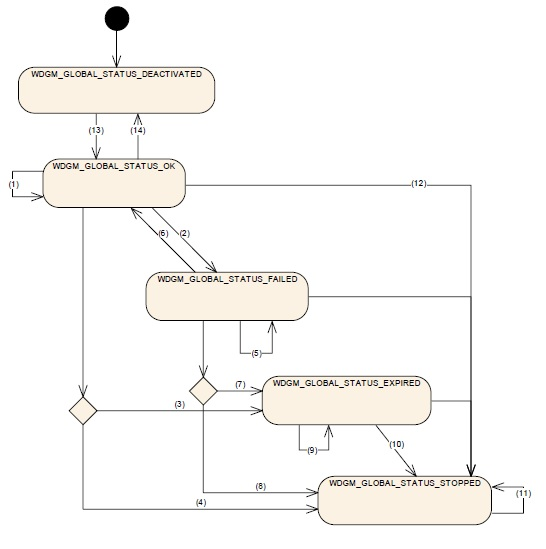
\includegraphics{pictures/globalstatuses.jpg}
  \end{center}
  \caption{State diagram that shows possible transitions between states}
  \label{FIG:GLOBALSTATUSES}
\end{figure}

\section{Configurations}
The watchdog manager (WdgM) was tested using three different
configurations. The configurations were of different complexity. One
was a minimal configuration, one an example configuration and one was
a live configuration, used in actual implementations.

Because there is only a small number of commands that influences the
state transitions, those commands were tweaked and therefore was
generated more often. On the other hand, all get-functions were
tweaked to not be generated as often.

\subsection{BSI}
As a highly simplified configuration, \emph{BSI} gives in some sense
good results.  Using this configuration the WdgM never visited the
absorbing state according to figure \ref{FIG:GLOBALSTATUSES}. However,
looking at the state transitions, as seen in figure
\ref{FIG:STATUSES_BSI} and table \ref{TABLE:STATUSES_BSI}, only two
states are visited. This happens because the configuration is to
simple, it is actually impossible to hit any other states than
\lstinline!WDGM_GLOBAL_STATUS_OK! or
\lstinline!WDGM_GLOBAL_STATUS_DEACTIVATED!. There are no checkpoints
or supervision functions configured for the \emph{BSI} configuration.
It is easy to run tests using this configuration but it does not by it
self, fully test the code because most of the specification
requirements will never be tested. The untested requirements are
mainly requirements for supervision functions that are, according to
the configuration, never executed. Those untested requirements also
leaves other requirements untested because the watchdog manager never
reaches a state when those other requirements must hold.

%% TODO: Dela upp grafer i mindre delar, exempelvis getters vs setters
%% och positive vs negative testing
\begin{figure}[!ht]
  \begin{center}
    \subfigure[Shows percentage of each possible command executed]{
      \label{FIG:COMMANDS_BSI}
      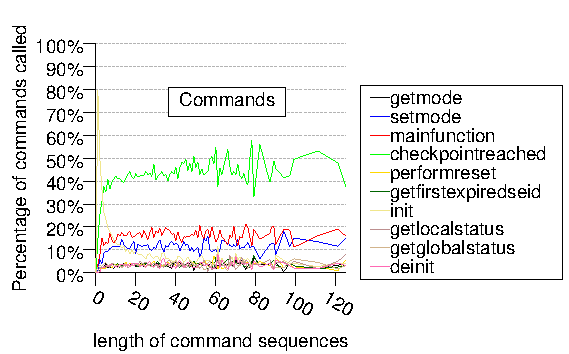
\includegraphics{generated_pictures/history_commands_bsi.pdf}
    }

    \subfigure[Shows percentage of each visited global status]{
      \label{FIG:STATUSES_BSI}
      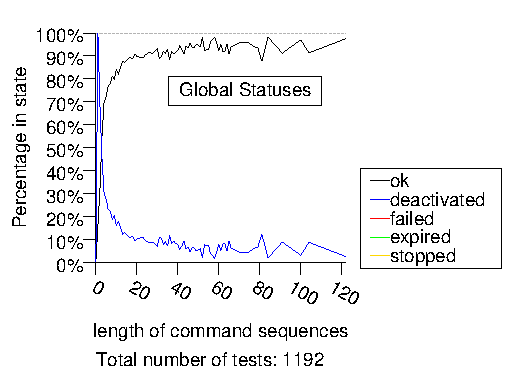
\includegraphics{generated_pictures/history_statuses_bsi.pdf}
    }
  \end{center}
  \caption{Some statistics of the BSI minimal configuration.}
  \label{FIG:BSI}
\end{figure}

\begin{table}[!ht]
  \caption{State transitions of the BSI configuration.}
  \label{TABLE:STATUSES_BSI}
  
    \begin{tabular}{r|ccccc}
        \hline
        \multicolumn{6}{c}{Number of tests: 2850} \\
        \hline
        \backslashbox{From}{To}
                    & DEACTIVATED & EXPIRED & FAILED & OK & STOPPED \\
        \hline
        DEACTIVATED & \bf{02.23}\% & 00.00\%       & 00.00\%       & \bf{09.12}\% & 00.00\% \\
        EXPIRED     & 00.00\%       & \bf{00.00}\% & 00.00\%       & 00.00\%       & \bf{00.00}\% \\
        FAILED      & 00.00\%       & \bf{00.00}\% & \bf{00.00}\% & \bf{00.00}\% & \bf{00.00}\% \\
        OK          & \bf{03.24}\% & \bf{00.00}\% & \bf{00.00}\% & \bf{85.41}\% & \bf{00.00}\% \\
        STOPPED     & 00.00\%       & 00.00\%       & 00.00\%       & 00.00\%       & \bf{00.00}\%
      \end{tabular}
    

\end{table}

Figure \ref{FIG:COMMANDS_BSI} shows how many times a certain command
was generated versus the length of the command sequence that was
generated. E.g. the function \lstinline!WdgM_CheckpointReached! was
generated in average a little more than 40\% of all calls. This is
because, in any other configuration, the supervision functions demand
that a certain number of checkpoints is reached before the next main
function is called\footnote{This is however not completely true, but
it gives the general idea.}. There is also a dependency the other way
around; the main function has to be called a certain number of times
before \lstinline!WdgM_CheckpointReached! is called on a certain
supervised entity. This is why the main function also has quite high
proportions. Other functions that stands out is
\lstinline!WdgM_SetMode! and \lstinline!WdgM_Init!.
\lstinline!WdgM_Setmode! is called because different modes can have
different supervision functions and supervised entities. That is why
we need to call this function often. It should retain the states of
supervised entities that is activated in the new mode and should reset
the local state if the entity is deactivated in the new mode. The
function \lstinline!WdgM_Init! is in contrast called lesser and lesser
times. This function is only needed when the global state is
deactivated. It has more likelihood to be generated among the first
commands in the command sequence, or right after a
\lstinline!WdgM_DeInit! deactivation call.


\subsection{Freescale}
The Freescale configuration is, compared to BSI, a more realistic
configuration.  All supervision algorithms are configured and there
are both external and internal graphs for logical supervision. It is
also one of the configurations that is actively used in lab
environments. The state machine for the global status is totally
covered by running QuickCheck, see table
\ref{TABLE:STATUSES_FREESCALE} and figure
\ref{FIG:STATUSES_FREESCALE}. Locking at table \ref{TABLE:STATUSES_FREESCALE}
one can see that some transitions are done very seldom. This is due to a lot of
things must be fulfilled for those transitions to occur, which also highly depend on
the configuration supplied. Due to the randomness factor of QuickCheck such cases are
hard to reach.

%% TODO: Fyll på text, beskriv resultaten. Det är i dagsläget den
%% kortaste texten om konfigurationer, trots att det är den viktigaste
%% konfigurationen.

\begin{figure}[!ht]
  \begin{center}
    \subfigure[Shows percentage of each possible command executed]{
      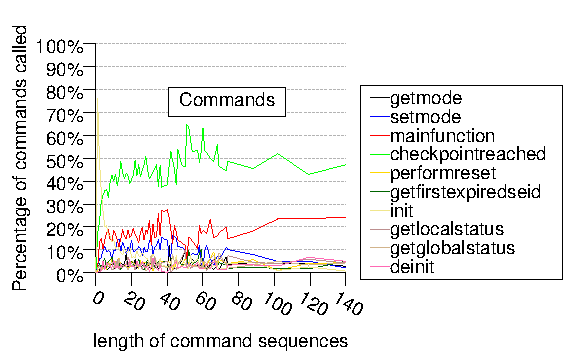
\includegraphics{generated_pictures/history_commands_freescale.pdf}
      \label{FIG:COMMANDS_FREESCALE}
    }
    \subfigure[Shows percentage of all visited global status]{
      \label{FIG:STATUSES_FREESCALE}
      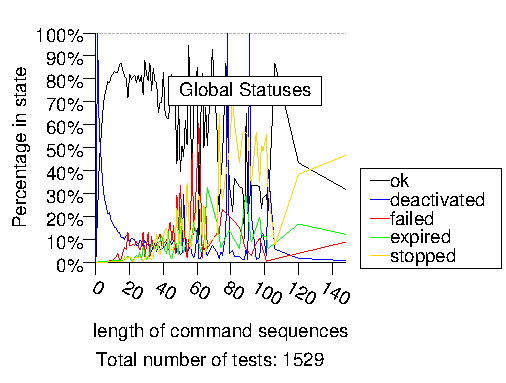
\includegraphics{generated_pictures/history_statuses_freescale.pdf}
    }
  \end{center}
  \caption{Some statistics for the Freescale configuration.}
  \label{FIG:FREESCALE}
\end{figure}

\begin{table}[!ht]
  \caption{State transitions of the Freescale configuration.}
  \label{TABLE:STATUSES_FREESCALE}
  
    \begin{tabular}{r|ccccc}
        \hline
        \multicolumn{6}{c}{Number of tests: 1023} \\
        \hline
        \backslashbox{From}{To}
                    & DEACTIVATED & EXPIRED & FAILED & OK & STOPPED \\
        \hline
        DEACTIVATED & \bf{02.43}\% & 00.00\%       & 00.00\%       & \bf{08.32}\% & 00.00\% \\
        EXPIRED     & 00.00\%       & \bf{03.36}\% & 00.00\%       & 00.00\%       & \bf{00.11}\% \\
        FAILED      & 00.00\%       & \bf{00.17}\% & \bf{07.77}\% & \bf{00.12}\% & \bf{00.11}\% \\
        OK          & \bf{02.56}\% & \bf{00.18}\% & \bf{00.87}\% & \bf{69.53}\% & \bf{00.12}\% \\
        STOPPED     & 00.00\%       & 00.00\%       & 00.00\%       & 00.00\%       & \bf{04.34}\%
      \end{tabular}
    

\end{table}

\subsection{Example}
The example configuration is somewhat more complex than the Freescale
configuration. This is because it supports all functionality of an
configuration. Because of the complexity, some transition is harder or
even impossible to reach. Noticeable is that the transition from the
state \lstinline!WDGM_GLOBAL_STATUS_FAILED! to the state
\lstinline!WDGM_GLOBAL_STATUS_OK! according to figure
\ref{FIG:GLOBALSTATUSES} is never made, see table
\ref{TABLE:STATUSES_EXAMPLE}. The reason for that is that the alive
functions must fail once and then continue without failures.
\begin{figure}[!ht]
  \begin{center}
    \subfigure[Shows percentage of each possible command executed]{
      \label{FIG:COMMANDS_EXAMPLE}
      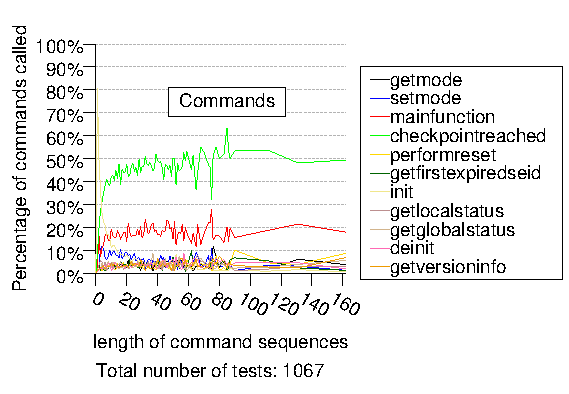
\includegraphics{generated_pictures/history_commands_example.pdf}
    }

    \subfigure[Shows percentage of all visited global status]{
      \label{FIG:STATUSES_EXAMPLE}
      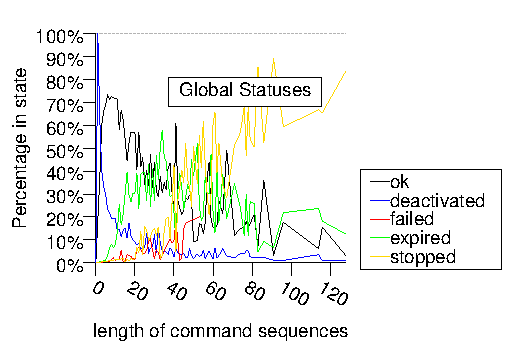
\includegraphics{generated_pictures/history_statuses_example.pdf}
    }
  \end{center}
  \caption{Some statistics for the Example configuration}
  \label{FIG:EXAMPLE}
\end{figure}

\begin{table}[!ht]
  \caption{State transitions of the Example configuration}
  \label{TABLE:STATUSES_EXAMPLE}
  
    \begin{tabular}{r|ccccc}
        \hline
        \multicolumn{6}{c}{Number of tests: 3877} \\
        \hline
        \backslashbox{From}{To}
                    & DEACTIVATED & EXPIRED & FAILED & OK & STOPPED \\
        \hline
        DEACTIVATED & \bf{02.59}\% & 00.00\%       & 00.00\%       & \bf{07.81}\% & 00.00\% \\
        EXPIRED     & 00.00\%       & \bf{24.77}\% & 00.00\%       & 00.00\%       & \bf{00.81}\% \\
        FAILED      & 00.00\%       & \bf{00.12}\% & \bf{02.87}\% & \bf{00.00}\% & \bf{00.04}\% \\
        OK          & \bf{01.68}\% & \bf{02.50}\% & \bf{00.39}\% & \bf{40.22}\% & \bf{00.14}\% \\
        STOPPED     & 00.00\%       & 00.00\%       & 00.00\%       & 00.00\%       & \bf{16.07}\%
      \end{tabular}
    

\end{table}

\section{Handle bugs in the C code}
\label{sec:handlebugs}
There is a number of possible ways to handle bugs when QuickCheck
encounters them. The problem is that QuickCheck generates arbitrary
command sequences, it cannot ``save'' an error and proceed to find the
next error. Either the C-code or the model needs to be adjusted.  The
best way, with the model in mind, would often be to let a third party
correct the discovered bugs. However this is time consuming because
the support line has often already much to do, and the releases
doesn't come that often.  Another way is to mock the faulty API
call. In other words simulate the output of the C-code, but then you
will only find one bug per function, strictly limiting the probability
to find bugs. There is a QuickCheck Erlang module for the purpose of
mocking C-code, see appendix \ref{APP:SEC:OTHERMODULES}. Then there is
two equally good methods. Either the Erlang model needs to have the
fault implemented, or the C-code needs to be fixed. There are pros and
cons with both methods. If the Erlang model introduce bugs, there may
be secondary failures which are not discovered. This could also happen
when correcting the C-code, but then more knowledge of the module is
needed, and some of the secondary failures can easier be avoided. It
also takes more time to get the extra knowledge of the C-code.

We choose to correct the C-code, because then we had direct feedback
and could discover where in the code the bugs were introduced.

\section{Statistics}
The distribution of API-calls seems, according to figure
\ref{FIG:COMMANDS_BSI}, \ref{FIG:COMMANDS_FREESCALE} and
\ref{FIG:COMMANDS_EXAMPLE}, to be the same for all configuration. The
arguments to the API calls is however different, even though it is not
seen in those plots.

\subsection{Important Functions}
The most interesting API calls is the ones that
modifies the internal state of the watchdog manager, see appendix
\ref{APP:API_CALLS}, namely \lstinline!WdgM_Init!,
\lstinline!WdgM_DeInit!, \lstinline!WdgM_SetMode!,
\lstinline!WdgM_MainFunction!, and
\lstinline!WdgM_CheckpointReached!. The reason for this is that they
will influence the result of following API calls.

The Init and DeInit functions can just change the global status
between two states, and should only change the state of the watchdog
when the watchdog is in either \lstinline!WDGM_GLOBAL_STATUS_OK! or
\lstinline!WDGM_GLOBAL_STATUS_DEACTIVATED!, according to figure
\ref{FIG:GLOBALSTATUSES}. If this happens they will change the
internal state of the watchdog independently of previous called
commands. The behaviour of these commands will therefor not vary much.

\lstinline!WdgM_SetMode! changes the mode, but should retain the
global and local statuses of the supervised entities. It should not be
possible to change the mode if the watchdog manager is in either
\lstinline!WDGM_GLOBAL_STATUS_EXPIRED! or
\lstinline!WDGM_GLOBAL_STATUS_STOPPED!.

The two remaining API-calls that needs to be discussed in details are
the main function and the checkpoint reached function. As can be seen
in figures \ref{FIG:COMMANDS_BSI}, \ref{FIG:COMMANDS_FREESCALE} and
\ref{FIG:COMMANDS_EXAMPLE}, they are also the two commands that are
called the most.

\subsubsection{\lstinline!WdgM_MainFunction!}
The \lstinline!WdgM_MainFunction! handles alive supervision
calculations, and the function \lstinline!WdgM_CheckpointReached!
handles the increasing of the alive counters, a certain number of
calls to \lstinline!WdgM_CheckpointReached! must be done before each
\lstinline!WdgM_MainFunction!. It does not end there. Each checkpoint
may have some logical supervision, so the order of the called
checkpoints is important as well. It is also possible to set deadline
supervision for a supervised entity. Both deadline supervision and
logical supervision is handled by

\subsubsection{\lstinline!WdgM_CheckpointReached!}
\lstinline!WdgM_CheckpointReached!. Deadline supervision demands that
a configured amount of time must have elapsed since the start
checkpoint was visited. Because AUTOSAR does not specify how the
handling of time should be implemented, see sections
\ref{SEC:CALLING_COMMANDS} and \ref{SEC:FUNCTIONAL_SAFETY_TIME}, we
implemented the model as the C-code, with the use of
\lstinline!WdgM_MainFunction!. This is possible because we know that
\lstinline!WdgM_MainFunction! is called periodically.

\section{Coverage}
\subsection{Erlang module}
%% TODO: Dubbelkolla dessa värden.
\newcommand{\linecoverage}{97.38\%}
\newcommand{\bullseyecoverage}{81\%}
The Erlang module \lstinline!cover! was used to calculate the line
coverage for the Erlang module. To get an idea of how many tests that
needed to be executed, before the line coverage of the Erlang module
converges against a certain value, the coverage was measured after
each executed test for every configuration.

\begin{figure}[!ht]
\begin{center}
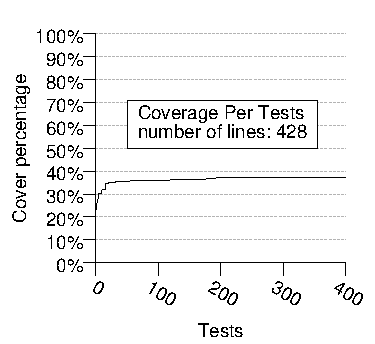
\includegraphics{generated_pictures/coverage_per_tests_bsi.pdf}
\end{center}
\caption{Coverage per tests using the BSI configuration}
\label{FIG:COV_PER_TESTS_BSI}
\end{figure}

\begin{figure}[!ht]
\begin{center}
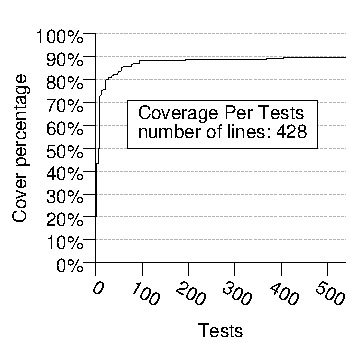
\includegraphics{generated_pictures/coverage_per_tests_freescale.pdf}
\end{center}
\caption{Coverage per tests using the Freescale configuration}
\label{FIG:COV_PER_TESTS_FREESCALE}
\end{figure}


\begin{figure}[!ht]
\begin{center}
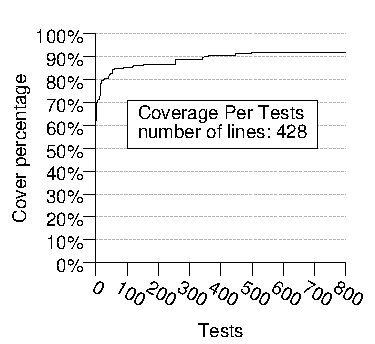
\includegraphics{generated_pictures/coverage_per_tests_example.pdf}
\end{center}
\caption{Coverage per tests using the Example configuration}
\label{FIG:COV_PER_TESTS_EXAMPLE}
\end{figure}

As can be seen in the figures \ref{FIG:COV_PER_TESTS_BSI},
\ref{FIG:COV_PER_TESTS_FREESCALE} and \ref{FIG:COV_PER_TESTS_EXAMPLE},
the example configuration takes the longest time before it
converges. It also becomes clear that the freescale configuration
needs more tests than the BSI configuration before it convergence. The
complexity of the configurations seem to play an important
part. This is not surprising because a more complex configuration may
drastically increase the state space.

The Erlang model is separated into a number of files. The results of the
coverages of these files, after running all configuration, can be seen in table
\ref{TABLE:COVERAGE}. This table lists the same modules as table \ref{TABLE:MODULES}.

The module \lstinline!wdgm_pre!
checks preconditions of the model state; constraining the model states
ability to change. This will affect the \lstinline!wdgm_next!
module. The \lstinline!wdgm_next! module changes the model state, and
is called after a call to the C-code is performed. Note that
\lstinline!wdgm_next! module are totally independent of the C-code,
see appendix \ref{APP:QUICKCHECK}. The \lstinline!wdgm_next! module
has two helper modules \lstinline!wdgm_main! and
\lstinline!wdgm_checkpointreached! which changes the model state if
the main function or the checkpoint reached function was the most
recently called functions in the C-code. The module
\lstinline!wdgm_post! checks that AUTOSAR specification holds, by
comparing the models state and the actual state of the C-code.

\begin{table}[!ht]
\caption{Shows coverage statistics generated by the Erlang module cover}.
\label{TABLE:COVERAGE}
\begin{center}
\begin{tabular}{l|l|l|l}
\hline
\multicolumn{4}{c}{Total line coverage \linecoverage} \\
\hline
module & total number of lines & lines covered & line coverage (\%)\\
\hline
wdgm\_helper            & 80  & 79 & 98.75\% \\
wdgm\_checkpointreached & 104 & 98 & 94.23\% \\
wdgm\_main              & 81  & 80 & 98.77\% \\
wdgm\_pre               & 19  & 19 & 100\%   \\
wdgm\_post              & 99  & 96 & 96.97\% \\
wdgm\_next              & 37  & 37 & 100\%
\end{tabular}
\end{center}
\end{table}

The total line coverage results is \linecoverage. The reason we don't
achieve 100\% code coverage depends on certain limitations. Some lines
can not be covered when the configuration parameter
\lstinline!WdgMDevErrorDetect! is true. On the other hand, if it is
false, then the C model will fail with a segmentation fault and the
Erlang model will not be covered any way. There are also a number of
implementation specific lines, which an other C code model might
reach but the one that we had. There is also places that depended on
the configuration to be more simple. A good idea is to supply
configurations that only has specific supervision functions
configured. Then it should be possible to prioritize only that
supervision function and get better coverages.

\subsection{C-code}
Bullseye Coverage was used to analyse the coverage of the C-code. The
results show that the decision coverage is over {\bullseyecoverage}
and all functions except for two is covered, see figure
\ref{FIG:BULLSEYE}. The reason that there are functions which are not
covered, is that one of the functions is deprecated and the other is a
support function to that function. One of our limitations were to not
implemented deprecated functions into Erlang code.  The missing
condition/decision coverages in the C-code are for example checks for
null pointers, some of which never evaluated to false. Many checks
seems to be redundant and impossible to evaluate to true, if one
excludes the possibility of hardware failures or other failures which
may corrupt the memory of the watchdog manager. There is as well
branches and conditions regarding the \lstinline!WdgMDevErrorDetect!
configuration parameter, which if turned off resulted in a
segmentation fault.

The coverage statistics shown in figure \ref{FIG:BULLSEYE} is
constructed using three configuration. Using several configurations
gave better results since some code is impossible to reach if not
certain configuration parameters are set.

\begin{figure}[!ht]
  \setlength\fboxsep{0pt}
  \setlength\fboxrule{0.5pt}
  \fbox{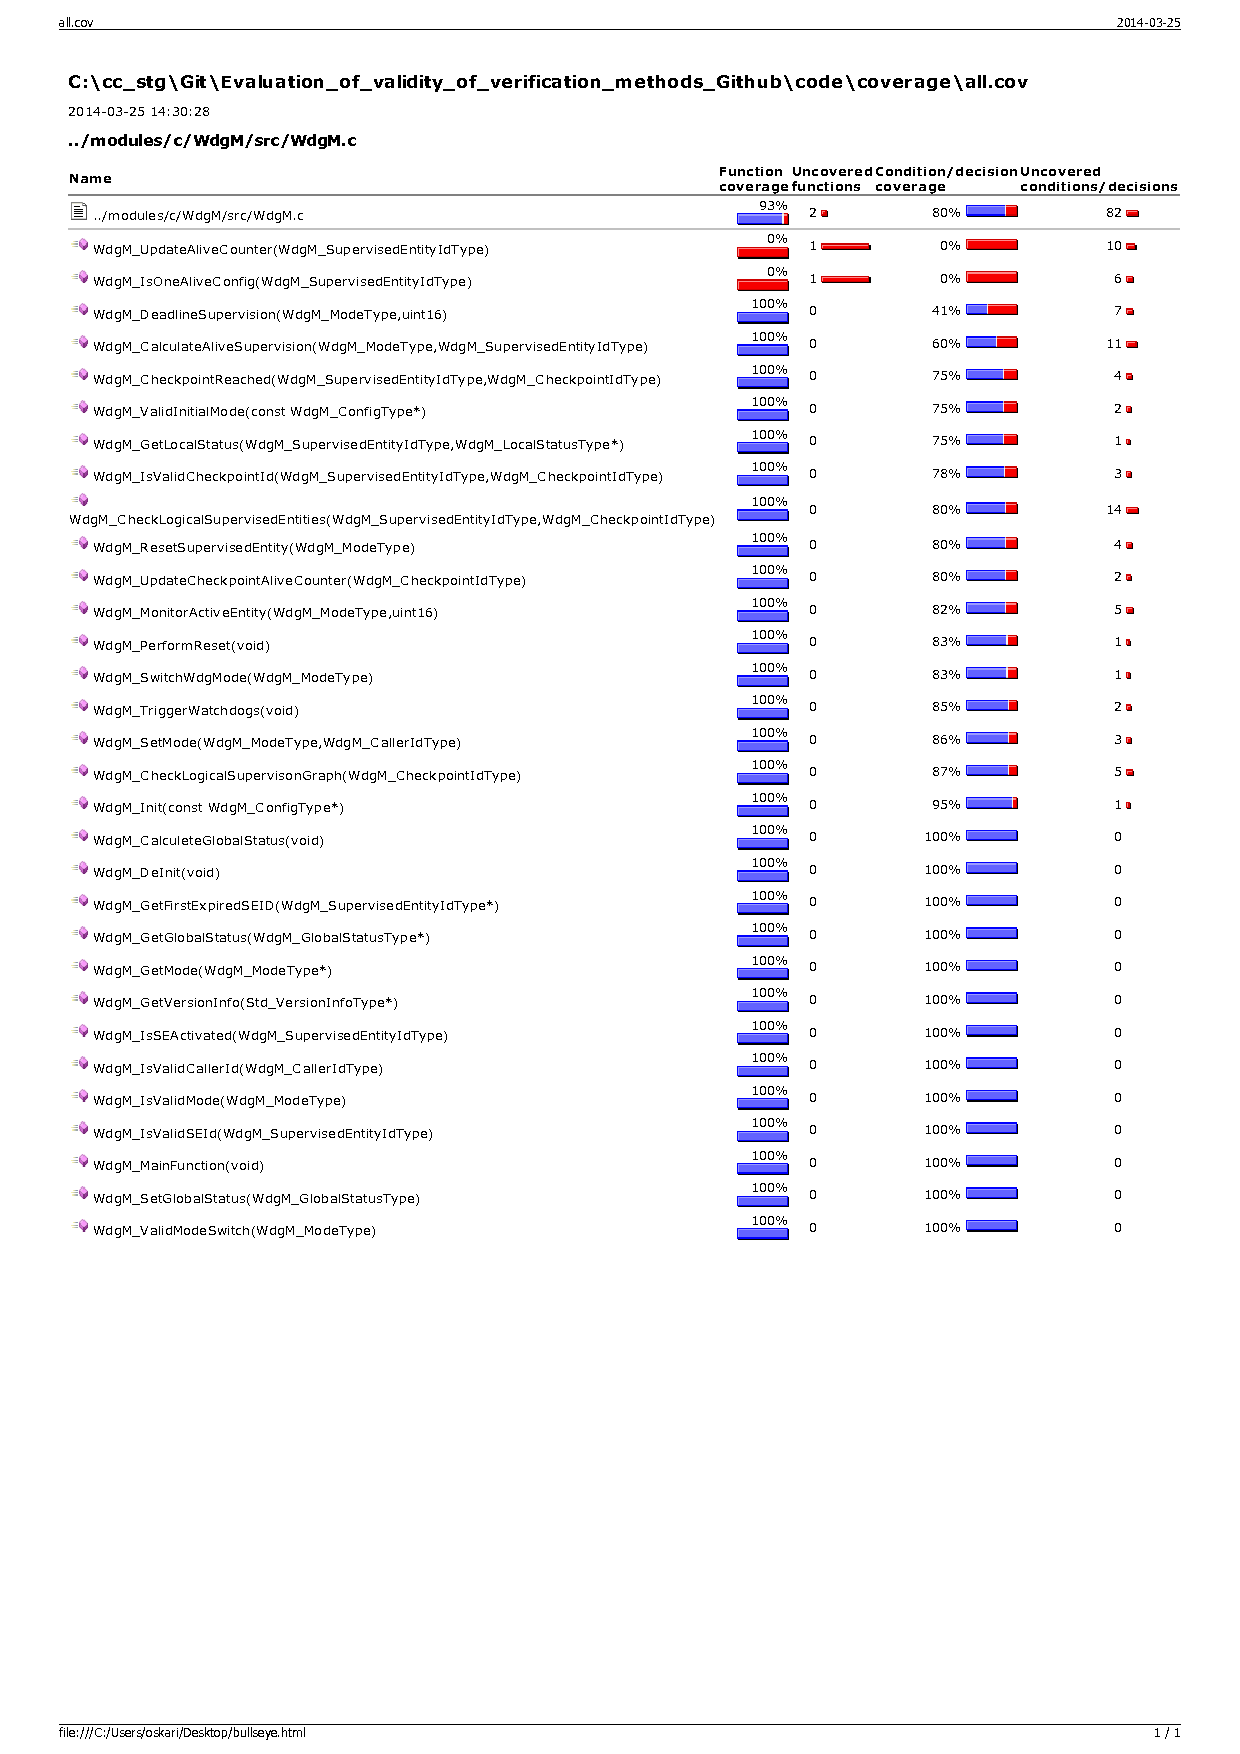
\includegraphics[keepaspectratio, width=\linewidth, clip=true, trim=1cm 8.5cm 1cm 2.7cm, scale=0.75]{generated_pictures/bullseye-coverage}}
  \caption{Shows coverage statistics generated by Bullseye Coverage}
  \label{FIG:BULLSEYE}
\end{figure}


\section{Functional Safety analysis}
The $V$ model used by ISO~26262 requires that a certain work flow is
taken into consideration during the whole development process. It is
therefor hard to analyze code that is written without the standard in
consideration and then examine if it fulfills that standards
requirements.

Since one important part of the functional safety concept is that it
must be taken in consideration during the whole development process,
one can not simply say that QuickCheck makes it possible to acquire
functional safety. There must first be a number of assumptions. If
every development step before the implementation of the watchdog
manager satisfies the requirements for functional safety, one also
must follow the same constraints in the remaining part of the
development life cycle to achieve functional safety. If this is
assumed, there is still one important assumption left before one can
reason about how QuickCheck can benefit. This assumption is based on
that the model for the watchdog manager is correct, namely the AUTOSAR
specification.

\subsection{AUTOSAR}
Due to the informal syntax of AUTOSAR it is not good fitted for
functional safety, since the informal syntax makes it possible for
different interpretation. To be able to reach the requirements for a higher
ASIL classification, AUTOSAR modules must be interpreted dependently. In other
means they must agree on the same model.

One way of doing this is to interpret AUTOSAR in a model based
language like SPIN and check that the model, after transforming it
into formal syntax, is valid. The model in itself should then not
contain any bugs.

This can also be done using QuickCheck but, in a functional safety
point of view, it seems pointless to test the actual C code before
there is assurance for that the model actually is correct according to
formal syntax.

C in itself is also a formal language but C is not good fitted to
formally defining the actual requirements of AUTOSAR. This is for
instance because of its low level nature.

In this thesis a defined AUTOSAR model already existed, written in C
code, and then an other model was later implemented in Erlang and
compared against the first model. A better work flow, with functional
safety in mind, had been to define AUTOSAR in a model based language
and check that this model holds. Then implement the actual C-code
following the formal notation of the previous constructed
model. Implementing the C-code would be easier because then there are
no room for different interpretations. After the C code is
implemented, write the model in Erlang following the formal model
written in the model based language. Then there are again no room for
different interpretations. After the two implementations of the model,
compare those using QuickCheck. If there are no bugs, then the
original model was translated into C code correctly.

The proposed work flow would require a lot of work which, is beyond the scope of
this thesis. For example the C-code needs to be rewritten.

\subsubsection{Development error detection}
\label{SEC:DEVERRORDETECT}
It was discovered that it existed a configuration parameter,
\lstinline!WdgMDevErrorDetect!, which would turn off functional safety
checks. This made the C-code crash with segmentation fault as soon as
negative testing was performed. This could for example be null pointers or
improper identification numbers. AUTOSAR is not specified enough for
the parameter \lstinline!WdgMDevErrorDetect!  to be switched off. With
functional safety in mind, this parameter must be on!

\subsubsection{Definition of time}
\label{SEC:FUNCTIONAL_SAFETY_TIME}
In AUTOSAR time is specified as seconds and there are two functions that need to
keep track of the time. First it is the main function that needs to be scheduled
periodically by the runtime environment. This is done with a configuration
parameter given for each mode. Time is also needed for deadline supervision. In
deadline supervision when a start checkpoint is reached, a timer should
start. If the final checkpoint is not reached within the configured time
marginal, then the deadline supervision for the supervised entity with the given
checkpoint will fail. Because it is known that \lstinline!WdgM_MainFunction! should
be called periodically, it could be used for the measurements of time. For each
call of \lstinline!WdgM_MainFunction! tick a ``time'' counter.


\subsection{Fulfilled ISO~26262 requirements}
ISO~26262 mention several several requirements that QuickCheck will be able to
fulfil. Aside from general requirements like that a ''safety plan'' should be
available, there are tests in which the hardware should be taken in
consideration. This is beyond the scope of this thesis and can also not be
tested using QuickCheck. There are also tests that needs several modules
implemented to make any sense. Such tests have not been executed, since only the
watchdog manager module has been tested, but should be possible to run after
implementing more modules in Erlang code. QuickCheck has a module for mocking C
code, see appendix \ref{SEC:QuickCheckIntro}, which could possible also be used
for running such tests.

\subsection{Confidence interval}

%% how certain is the verification

%% LoC
%% right side of pipe:  without blank lines and comments
%% *.c files: 3271 | 1736
%% *.h files: 18964 | 10942
%% total c-code: 22235 | 12678
%% *.erl: 2006 | 1470
%% *.hrl: 68 | 64
%% total erlang: 2074 | 1534


\subsection{Measurements of the state space}
One way when trying the measure the state space is to collect
statistical data during the execution of the tests. It is hard to say
much about the whole systems state space since it is very large, due
to the state explosion problem. In the case of an AUTOSAR module the
state space also varies on the configuration in use, since features
and supervision features can be configured.  However looking at
certain parts that are considered to be important for the system, much
more can be said. For instance when examining the internal graphs of
the watchdog manager, one can easily see that every node in those
graphs are visited.

Measuring the code coverage can in itself tell if important parts of
the state space are covered or not. This is possible because the parts
of the code that changes the state of the watchdog manager are not
covered. These parts can however be dead or redundant code, in the
worst case, if something unexpected happens to the hardware, which is
beyond this thesis. Total code coverage is hard, or may be even
impossible to reach.  Even if all lines of code in for example an
algorithmic part of the watchdog manager are covered this algorithm
may not be totally verified. This is because the state are dependent
of actual values of variables.
